\scanpage{421}
\mspage{512}

or that $\sigma$ as an element of $T_\sigma$
is in $ST_\sigma$ i.e. in the center of $\mathcal M_{\rho,\sigma}^{\circ}$.
So in this case we find a homomorphism
\diagram{\(\displaystyle
(54)\quad\left\{
\begin{gathered}
\begin{tikzcd}[ampersand replacement=\&,column sep=large,row sep=large]
\mathbb Z/6\mathbb Z\times\mathbb Z/4\mathbb Z \arrow[r] \&
\uline{\operatorname{Centr}}(\mathcal M_{\rho,\sigma}^{\circ})\\
(i,j) \arrow[r] \& i_\rho(\rho^i)i_\sigma(\sigma^j)
\end{tikzcd}
\end{gathered}\right.
\)}
(where we define $i_\rho,i_\sigma$ among the
\deleted{\unsure{four}}\inserted{three} canonical morphisms
\[
\deleted{(55)\quad\unsure{i_B}:B'_0\longrightarrow
\mathcal M_{\rho,\sigma}[0]\subset\mathcal M_{\rho,\sigma}}
\]
\diagram{\(\displaystyle
(55)\quad\left\{
\begin{gathered}
\begin{tikzcd}[ampersand replacement=\&,column sep=large,row sep=small]
i_\rho:S'T_\rho \arrow[r] \& \mathcal M_{\rho,\sigma}(0)
\arrow[r,phantom,"{\subset}" description] \& \mathcal M_{\rho,\sigma}\\
i_\sigma:\unsure{SN'_\sigma} \arrow[r] \& \mathcal M_{\rho,\sigma}(0)
\arrow[r,phantom,"{\subset}" description] \& \mathcal M_{\rho,\sigma}\\
i_G:SG\simeq\widetilde{\mathcal G}_{\rho,\sigma}^{+}
\arrow[r] \& \mathcal M_{\rho,\sigma}, \&
\end{tikzcd}
\end{gathered}\right.\qquad)
\)}
whose image, for $2$ invertible on $S$, contains
contains the image of $\mu_2\times\mu_2\times1$ in (48).
For $2$ invertible on $S$, the homomorphism (53) is a monomorphism
(but not in characteristic $2$, of course). Over the absolute base $\mathbb Z$,
we have moreover, in the modular case
\[
(56)\qquad
\left\{\begin{aligned}
\mathcal T_{\rho,\sigma}(\mathbb Z)&\simeq
T_\rho(\mathbb Z)\times N'_\sigma(\mathbb Z)
\simeq\mathbb Z/6\mathbb Z\times\mathbb D_4\\
\mathcal M_{\rho,\sigma}(\mathbb Z)&\simeq
\mathcal T_{\rho,\sigma}(\mathbb Z)\mathbin{.}\operatorname{Sl}(2,\mathbb Z)
\end{aligned}\right.
\]
\inserted{$\frac12$ direct product,
$\unsure{\mathbb D|\mathcal B|\mathcal T}_{\rho,\sigma}\simeq
\mathbb Z/6\mathbb Z\times\mathbb D_4$ operating via the character
\diagram{\begin{tikzcd}[ampersand replacement=\&,column sep=large]
\mathbb D_4 \arrow[r,"{\varepsilon_2}"] \&
\mathbb Z/2\mathbb Z\simeq\unsure{(1,\tau_\infty)|\{1,\tau_\infty\}}
\end{tikzcd}}
$\tau_\infty$ operating on $\operatorname{Sl}(2,\mathbb Z)$ by
automorphism induced by the matrix
\[
\tau_\infty=\begin{pmatrix}-1&0\\0&1\end{pmatrix}
\]
}

\margin{\figure{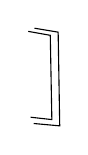
\begin{tikzpicture}[x=1cm,y=1cm]
\draw (0,1.15)--(.28,1.10)--(.30,.03)--(.03,.06);
\draw (.08,1.19)--(.38,1.14)--(.40,-.05)--(.07,-.02);
\end{tikzpicture}}}

\par\noindent 420

\scanpage{422}

\margin{the homomorphisms $\Theta,\widetilde\Theta$
$\Theta^\circ,\widetilde\Theta^\circ$}

\textcircled{\(4^\circ\)}\quad We define a homomorphism
\diagram{\begin{tikzcd}[ampersand replacement=\&,column sep=huge]
\text{(57)}\quad\mathcal M_{\rho,\sigma} \arrow[r,"{\Theta}"] \& G
\end{tikzcd}}
\[
\Theta\mid\widetilde{\mathcal G}_{\rho,\sigma}^{+}\simeq SG
\quad\text{is the identity}
\]
\[
\Theta\mid\mathcal M_{\rho,\sigma}(0)\subset
T_0\times T_\rho\times N'_\sigma
\quad\text{given by}\quad
\Theta(\underline u,\underline a,\underline b)=\underline u
\]
hence
\[
(58)\qquad
\Theta\mid\mathcal M_{\rho,\sigma}[0]\subset
B'_0\times T_\rho\times N'_\sigma
\quad\text{given by}\quad
\Theta(\underline u,\underline a,\underline b)=\underline u
\]

We have
\diagram{\begin{tikzcd}[ampersand replacement=\&,column sep=large,row sep=large]
\text{(59)}\quad\deleted{\operatorname{Ker}\Theta=}
\arrow[d,phantom,"{\deleted{\simeq}}"{description,rotate=90}]
\& \mathcal M_{\rho,\sigma}(0)
\arrow[r,phantom,"{\subset}" description]
\arrow[d,phantom,"{\cup}" description]
\arrow[dr,phantom,"{\text{Cartesian}}" description]
\& T_0\times T_\rho\times N'_\sigma
\arrow[d,phantom,"{\cup}" description]\\
\deleted{\unsure{\mathcal R|SG}}
\& \operatorname{Ker}\Theta
\arrow[r,phantom,"{\subset}" description]
\& 1\times T_\rho\times N'_\sigma
\end{tikzcd}}
\[
\begin{gathered}
\rotatebox{90}{$\simeq$}\quad
\left\{\left(1,
\underset{\substack{\rotatebox{90}{$\in$}\\\Gamma T_\rho}}{\underline a},
\underset{\substack{\rotatebox{90}{$\in$}\\\Gamma N'_\sigma}}{\underline b}
\right)\,\middle|\,\det\underline b=1,(\det\underline a)^2=1\right\}\\
\rotatebox{90}{$\simeq$}\quad S'T_\rho\times SN'_\sigma
\end{gathered}
\]
\inserted{where
$SN'_\sigma=\operatorname{Ker}(N'_\sigma\xrightarrow{\text{determinant}}\mathbb G_m)$}

Let
\[
(60)\qquad
\Theta^\circ=\Theta\mid\mathcal M_{\rho,\sigma}^{\circ}
\qquad\deleted{\text{\unsure{that we|we have}}}
\]
we find
\diagram{\begin{tikzcd}[ampersand replacement=\&,column sep=large,row sep=small]
\text{(61)}\quad1 \arrow[r] \& \operatorname{Ker}\Theta^\circ
\arrow[r] \arrow[d,phantom,"{\simeq}"{description,rotate=90}]
\& \operatorname{Ker}\Theta \arrow[r,"{(\varepsilon_3,\varepsilon_2)}"]
\& \mu_2\times\mu_2 \arrow[r] \& 1.\\
\& ST_\rho\times ST_\sigma
\arrow[d,phantom,"{\deleted{\simeq}}"{description,rotate=90}] \& \& \&\\
\& \deleted{\operatorname{Centr}} \& \& \&\\[-1.5ex]
\& \deleted{\bigl(\uline{\operatorname{Rad}}(\mathcal M_{\rho,\sigma}^{\circ})}
\arrow[d,phantom,"{\deleted{\simeq}}"{description,rotate=90}] \& \& \&\\
\& \deleted{\uline{\operatorname{Centr}}^\circ(\mathcal M_{\rho,\sigma}^{\circ})\bigr)}
\& \& \&
\end{tikzcd}}

Put
\[
(62)\qquad
S\mathcal R_{\rho,\sigma}^{\circ}
=1\times ST_\rho\times ST_\sigma
=\operatorname{Ker}\Theta^\circ
=(\operatorname{Ker}\Theta)\cap\mathcal M_{\rho,\sigma}^{\circ}
\]
which is a central subgroup of $\mathcal M_{\rho,\sigma}^{\circ}$
(it is

\par\noindent 421

\scanpage{423}
\mspage{513}

\deleted{\unsure{invariant}}\inserted{normal}
but not central in $\mathcal M_{\rho,\sigma}$ as a whole)

the group
\[
(63)\qquad
\mathcal M_{\rho,\sigma}/S\mathcal R_{\rho,\sigma}^{\circ}
=\mathcal M_{\rho,\sigma}^{\unsure{\natural}}
\]
is therefore an extension of $\mu_2\times\mu_2$ by
\[
\mathcal M_{\rho,\sigma}^{\circ}/S\mathcal R_{\rho,\sigma}^{\circ}
\overset{\mathrm{dfn}}{=}
\mathcal M_{\rho,\sigma}^{\circ\unsure{\natural}},
\]
isomorphic to $G$ via $\Theta^\circ$
(since $S\mathcal R_{\rho,\sigma}^{\circ}=\operatorname{Ker}\Theta^\circ$), hence
\diagram{\begin{tikzcd}[ampersand replacement=\&,column sep=large]
\text{(64)}\quad1 \arrow[r] \& G \arrow[r] \&
\mathcal M_{\rho,\sigma}^{\unsure{\natural}} \arrow[r] \&
\mu_2\times\mu_2 \arrow[r] \& 1,
\end{tikzcd}}
moreover the homomorphism
\diagram{\begin{tikzcd}[ampersand replacement=\&,column sep=large]
\Theta:\mathcal M_{\rho,\sigma} \arrow[r] \& G
\end{tikzcd}}
being trivial on $\mathcal R_{\rho,\sigma}$ passes to the quotient as
\diagram{\begin{tikzcd}[ampersand replacement=\&,column sep=large]
\text{(65)}\quad\Theta^{\unsure{\natural}}:
\mathcal M_{\rho,\sigma}^{\unsure{\natural}} \arrow[r] \& G,
\end{tikzcd}}
\unsure{whose} restriction to $G$ (via (64)) is the identity,
so we find, via (64),
\[
(66)\qquad
\mathcal M_{\rho,\sigma}^{\unsure{\natural}}\simeq
G\times\mu_2\times\mu_2.
\]
We thus find
\diagram{\begin{tikzcd}[ampersand replacement=\&,column sep=large,row sep=small]
\text{(67)}\quad1 \arrow[r] \& S\mathcal R_{\rho,\sigma}^{\circ}
\arrow[r] \arrow[d,phantom,"{\simeq}"{description,rotate=90}]
\& \mathcal M_{\rho,\sigma}
\arrow[r,"{(\Theta,\varepsilon_3,\varepsilon_2)}"] \&
\mathcal M_{\rho,\sigma}^{\unsure{\natural}}
\arrow[r] \arrow[d,phantom,"{\simeq}"{description,rotate=90}] \& 1.\\
\& ST_\rho\times ST_\sigma \& \& G\times\mu_2\times\mu_2 \&
\end{tikzcd}}

To see how
$\mathcal M_{\rho,\sigma}^{\unsure{\natural}}\simeq G\times\mu_2\times\mu_2$
operates on $ST_\rho\times ST_\sigma$, we
\deleted{consider the}\inserted{note that}\deleted{the image}
$\mathcal M_{\rho,\sigma}^{\circ}$ is the inverse image of
$G\simeq\mathcal M_{\rho,\sigma}^{\unsure{\natural}\circ}$
\deleted{subgroup}
in the extension (67), where $S\mathcal R_{\rho,\sigma}$ is central
in $\mathcal M_{\rho,\sigma}$, so $G$ operates trivially on it.

\par\noindent 422


\scanpage{424}

On the other hand we have
\diagram{\begin{tikzcd}[ampersand replacement=\&,column sep=large,row sep=small]
S\mathcal R_{\rho,\sigma}^{\circ}
\arrow[r,phantom,"{\subset}"{description}]
\arrow[d,phantom,"{\simeq}"{description,rotate=90}]
\& \mathcal M_{\rho,\sigma}(0)
\arrow[r,"{\text{epimorphism}}","{(\varepsilon_3,\varepsilon_2)}"']
\arrow[d,phantom,"{\cap}"{description}]
\& \mu_2\times\mu_2\\
ST_\rho\times ST_\sigma \& T_0\times T_\rho\times N'_\sigma \&
\end{tikzcd}}
and we find that $\mu_2\times\mu_2$ operates on
$S\mathcal R_{\rho,\sigma}$ via its second factor
(corresponding to
$\varepsilon_2(\underline u,\underline a,\underline b)
=\varepsilon_\sigma(\underline b)$), an $\varepsilon$ of the latter
($\varepsilon^2=1$) operates on
$S\mathcal R_{\rho,\sigma}\simeq ST_\rho\times ST_\sigma$
leaving the first factor untouched,
and operating on $T_\sigma$ hence on $ST_\sigma$ via
\diagram{\begin{tikzcd}[ampersand replacement=\&,column sep=large]
\text{(68)}\qquad\sigma \arrow[r] \& \varepsilon\sigma
\end{tikzcd}}
\margin{(compatible with the Hamilton--Cayley equation
$\sigma^2-\nu=0$ of $\sigma$)}

\deleted{We find in passing that the inverse image
 in $\mathcal M_{\rho,\sigma}$
\inserted{(or $\mathcal M_{\rho,\sigma}^{\circ}$)}
of the subgroup $\mathbb G_m\subset G$
center of $G$ \unsure{is none other than}
$\mathcal M_{\rho,\sigma}^{\unsure{\circ}}(0)^\circ$.}

\textcircled{\(5^\circ\)}\quad Let
\[
(69)\qquad
\begin{gathered}
\mathcal R_{\rho,\sigma}^{\circ}\quad
\text{inverse image of }\mathbb G_m\subset G\\
\text{in }\mathcal M_{\rho,\sigma}^{\circ}\text{ under }
\Theta:\mathcal M_{\rho,\sigma}^{\circ}\longrightarrow G
\end{gathered}
\]

\margin{It would be worthwhile to \unsure{begin}
right away with the introduction
of $\mathcal R_{\rho,\sigma}$ and the realization
(102) below of $\mathcal M_{\rho,\sigma}$,
in terms of amalgamated sums
of the products...\ cf.
\textcircled{\(6^\circ\)}.}

We thus have an extension structure on $\mathcal R_{\rho,\sigma}^{\circ}$
\diagram{\begin{tikzcd}[ampersand replacement=\&,column sep=large]
\text{(70)}\quad1 \arrow[r] \& S\mathcal R_{\rho,\sigma}^{\circ}
\arrow[r] \& \mathcal R_{\rho,\sigma}^{\circ}
\arrow[r] \& \mathbb G_m \arrow[r] \& 1.
\end{tikzcd}}
We will have
\[
\mathcal R_{\rho,\sigma}^{\circ}=
\left\{\left(
\underset{\substack{\rotatebox{90}{$\in$}\\\Gamma T_0}}{\underline u},
\underset{\substack{\rotatebox{90}{$\in$}\\\Gamma T_\rho}}{\underline a},
\underset{\substack{\rotatebox{90}{$\in$}\\\Gamma T_\sigma}}{\underline b}
\right)\cdot
\underset{\substack{\rotatebox{90}{$\in$}\\\Gamma SG}}{f}
\ \middle|\ 
\det u=\det\underline a=\det\underline b,\quad
\underline u f\in\Gamma\mathbb G_m
\right\}
\]
\inserted{i.e. $f=\lambda\underline u^{-1}$
 where $\lambda\in\Gamma\mathbb G_m$, $\lambda^2=\det u$}

\par\noindent 423